\documentclass[12pt, a4paper]{article}

%% Language and font encoding
\usepackage[english]{babel}
\usepackage[utf8x]{inputenc}
\usepackage[T1]{fontenc}
%\usepackage{palatino}
%\usepackage{newpxtext,newpxmath}
\usepackage{newtxtext,newtxmath}

%% Sets page size and margins
\usepackage[a4paper,top=2cm,bottom=2cm,left=2.5cm,right=2.5cm,marginparwidth=1.75cm]{geometry}
%\usepackage{fullwidth}

%% Useful packages
\usepackage{amsmath}
\usepackage{graphicx}
\graphicspath{{analysis}} %Setting the graphicspath
\usepackage[colorinlistoftodos]{todonotes}
\usepackage[colorlinks=true, allcolors=blue]{hyperref}
\usepackage{siunitx}
%\usepackage{booktabs} % used for tables exported from JASP
\usepackage[super]{nth}

%\usepackage[dvipsnames]{xcolor}
\newcommand{\note}[1] {{\textcolor{orange}{#1}}}
% \newcommand{\todo}[1] {{\textcolor{red}{#1}}}



%% Style
% make figure caption text smaller
% \usepackage[font=small,labelfont=bf, sf,textfont=sf]{caption}
\usepackage[font=small,labelfont=bf]{caption}
% **** REMOVE SECTION NUMBERING
\setcounter{secnumdepth}{0}

\usepackage{authblk}


%% Referencing
\usepackage[natbibapa, bibnewpage, doi]{apacite}
\usepackage{doi}
\renewcommand{\doitext}{} %fix for repeated "doi:" in references


\usepackage[figurename=Supplementary Figure]{caption}
%% I want the figure captions to start with "Supplementary Figure N: "
%\renewcommand{\figurename}{Supplementary Figure}


\title{{\normalsize \textsc{\textcolor{red}{Supplementary Material}}}\\ Still no link between temporal discounting and body composition}

\author{Benjamin T. Vincent}
%\author{Amy Parr}
\affil{School of Social Science, University of Dundee, Scotland, UK.}

\begin{document}

\maketitle

This document contains the supplementary figures. All data and code are available in the online Supplementary Material at the Open Science Foundation, \url{https://osf.io/vtf6j/}.
Bayesian moderation analyses were conducted using the PyMC3   package \citep{Salvatier:2016ki}. See the Methods of the main paper for more details.

% STUDY 1 ==============================

\begin{figure*} 
	\centering
	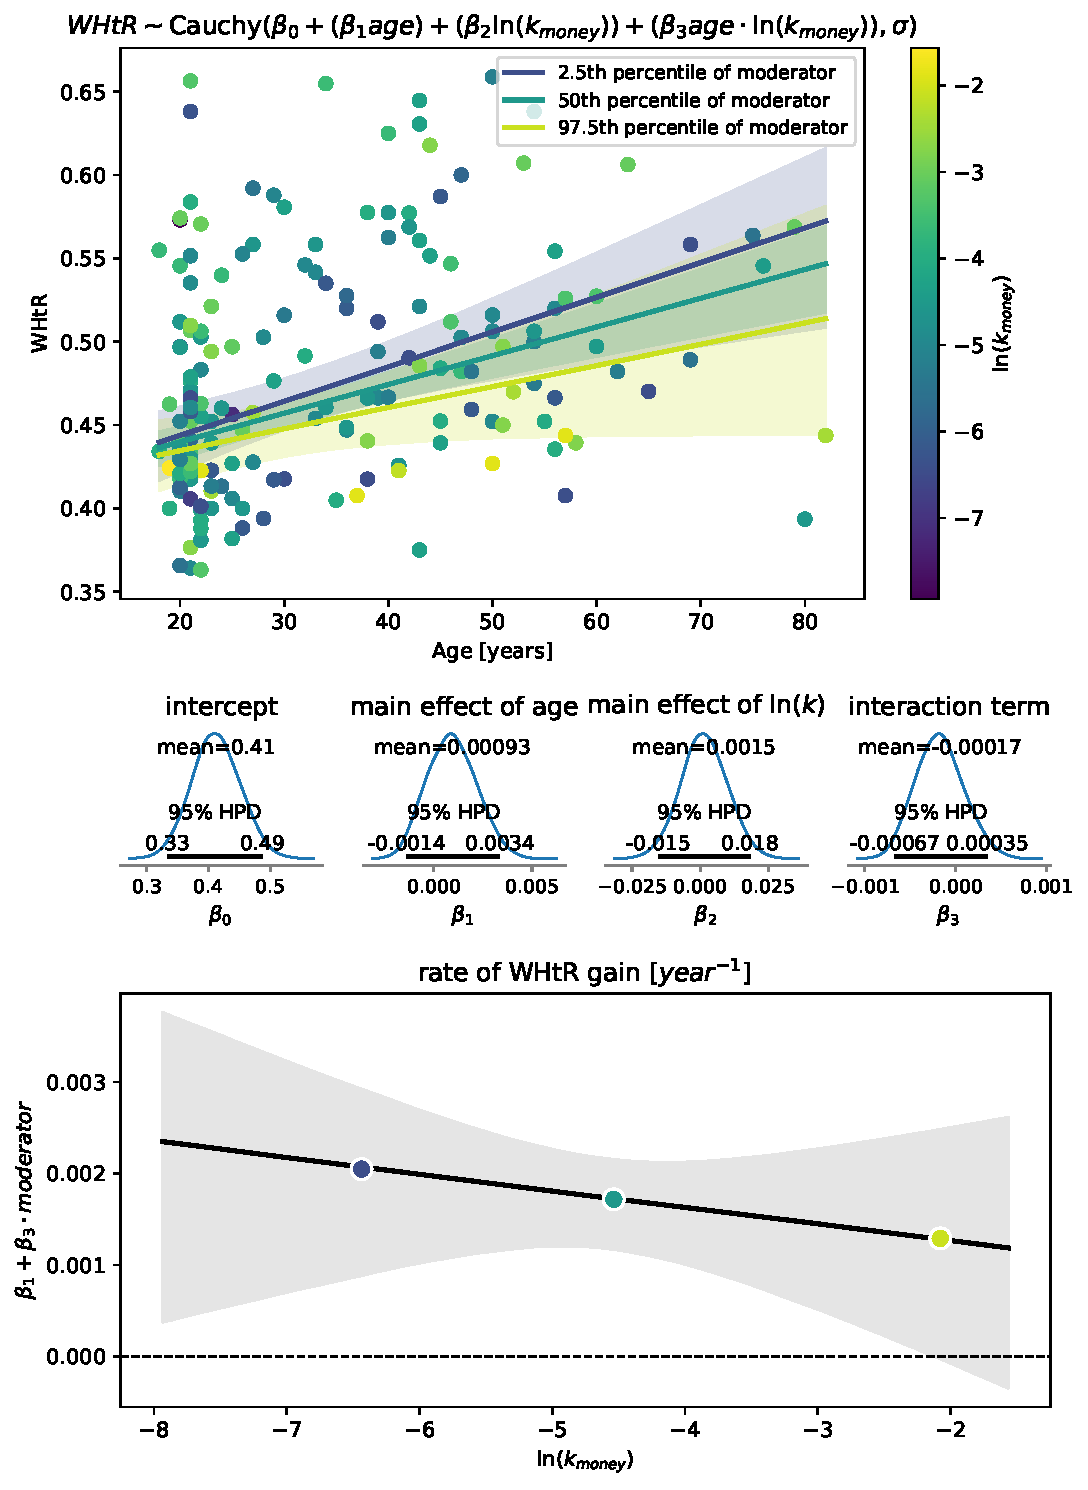
\includegraphics[width=0.8\textwidth]{analysis/study1 whtr~age*money.pdf} 
	\caption{Bayesian moderation analysis for Study 1 with age and discounting of money in predicting WHtR.}
	\label{fig:s1_whtr_money}
\end{figure*}


\begin{figure*} 
	\centering
	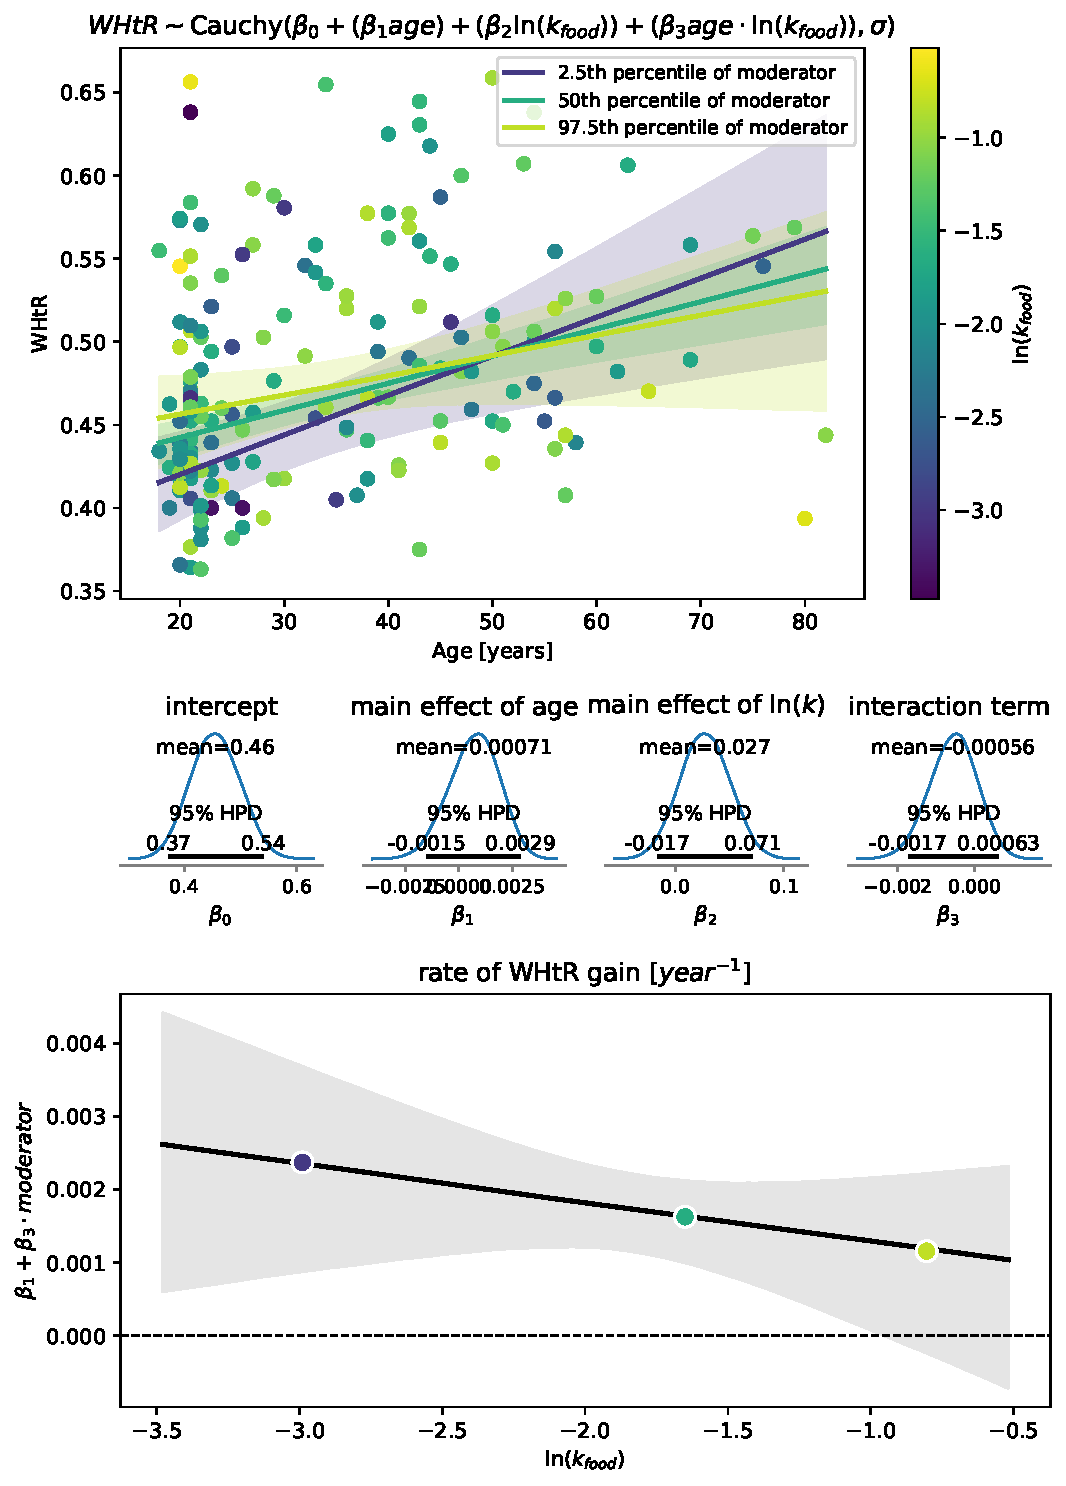
\includegraphics[width=0.8\textwidth]{analysis/study1 whtr~age*food.pdf} 
	\caption{Bayesian moderation analysis for Study 1 with age and discounting of food in predicting WHtR.}
	\label{fig:s1_whtr_food}
\end{figure*}

 
% STUDY 2 ==============================

\begin{figure*} 
	\centering
	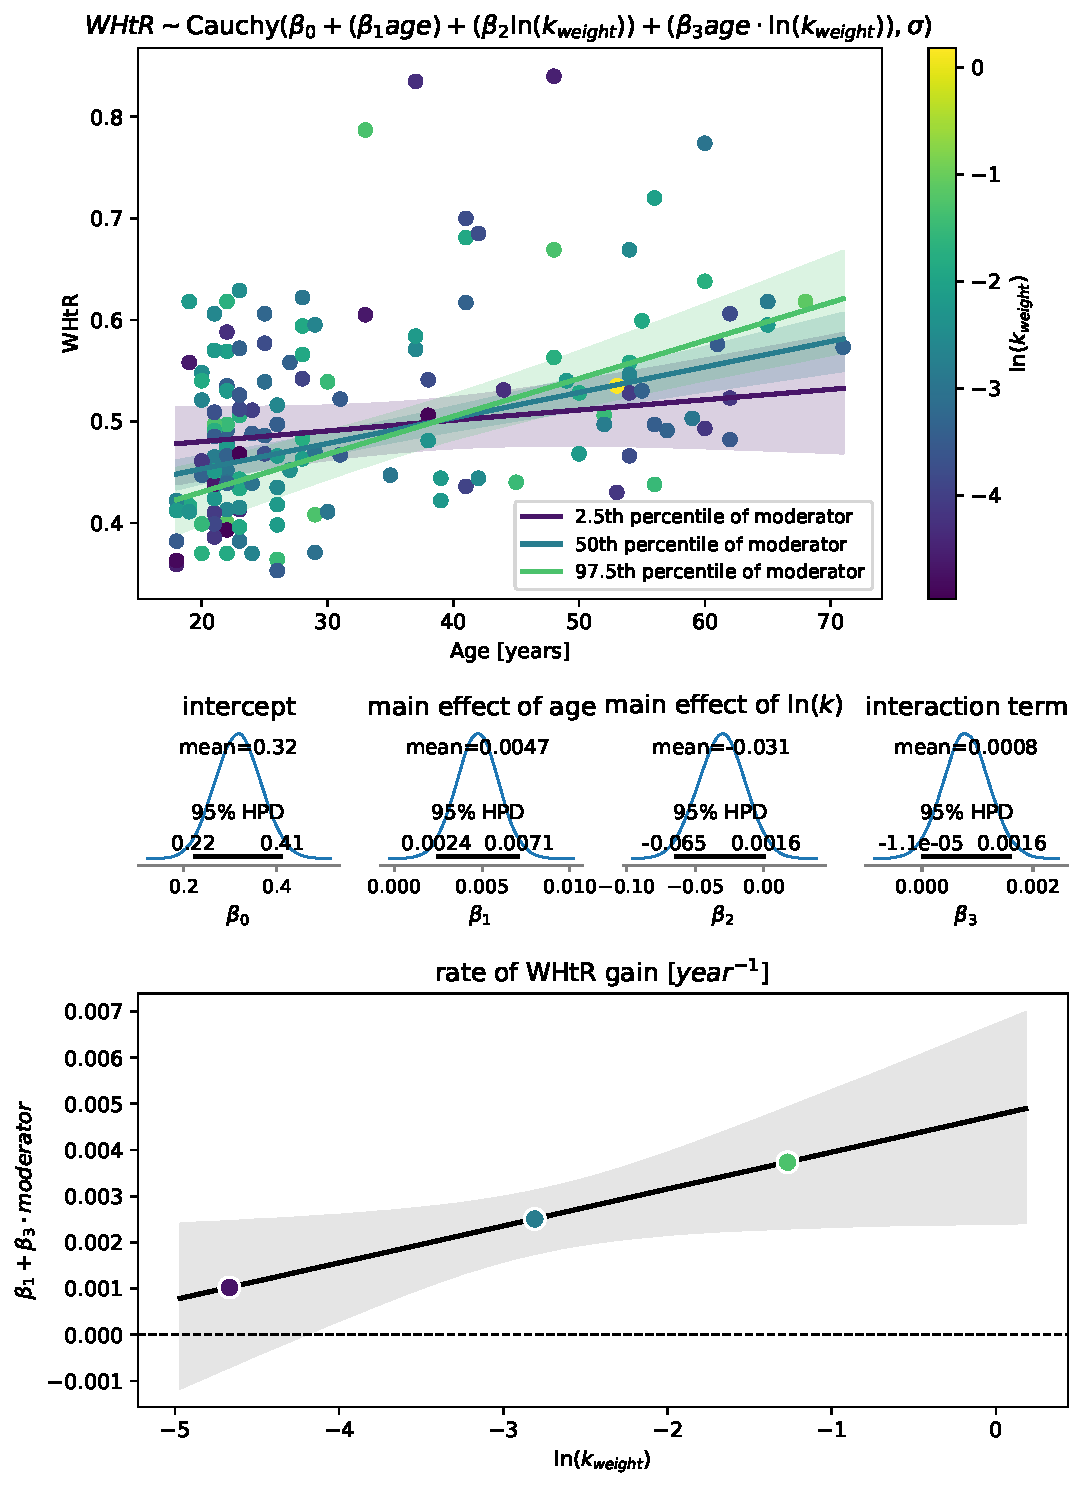
\includegraphics[width=0.8\textwidth]{analysis/study2 whtr~age*weight.pdf} 
	\caption{Bayesian moderation analysis for Study 2 with age and discounting of weight loss in predicting WHtR.}
	\label{fig:s2_whtr_weight}
\end{figure*}


\begin{figure*} 
	\centering
	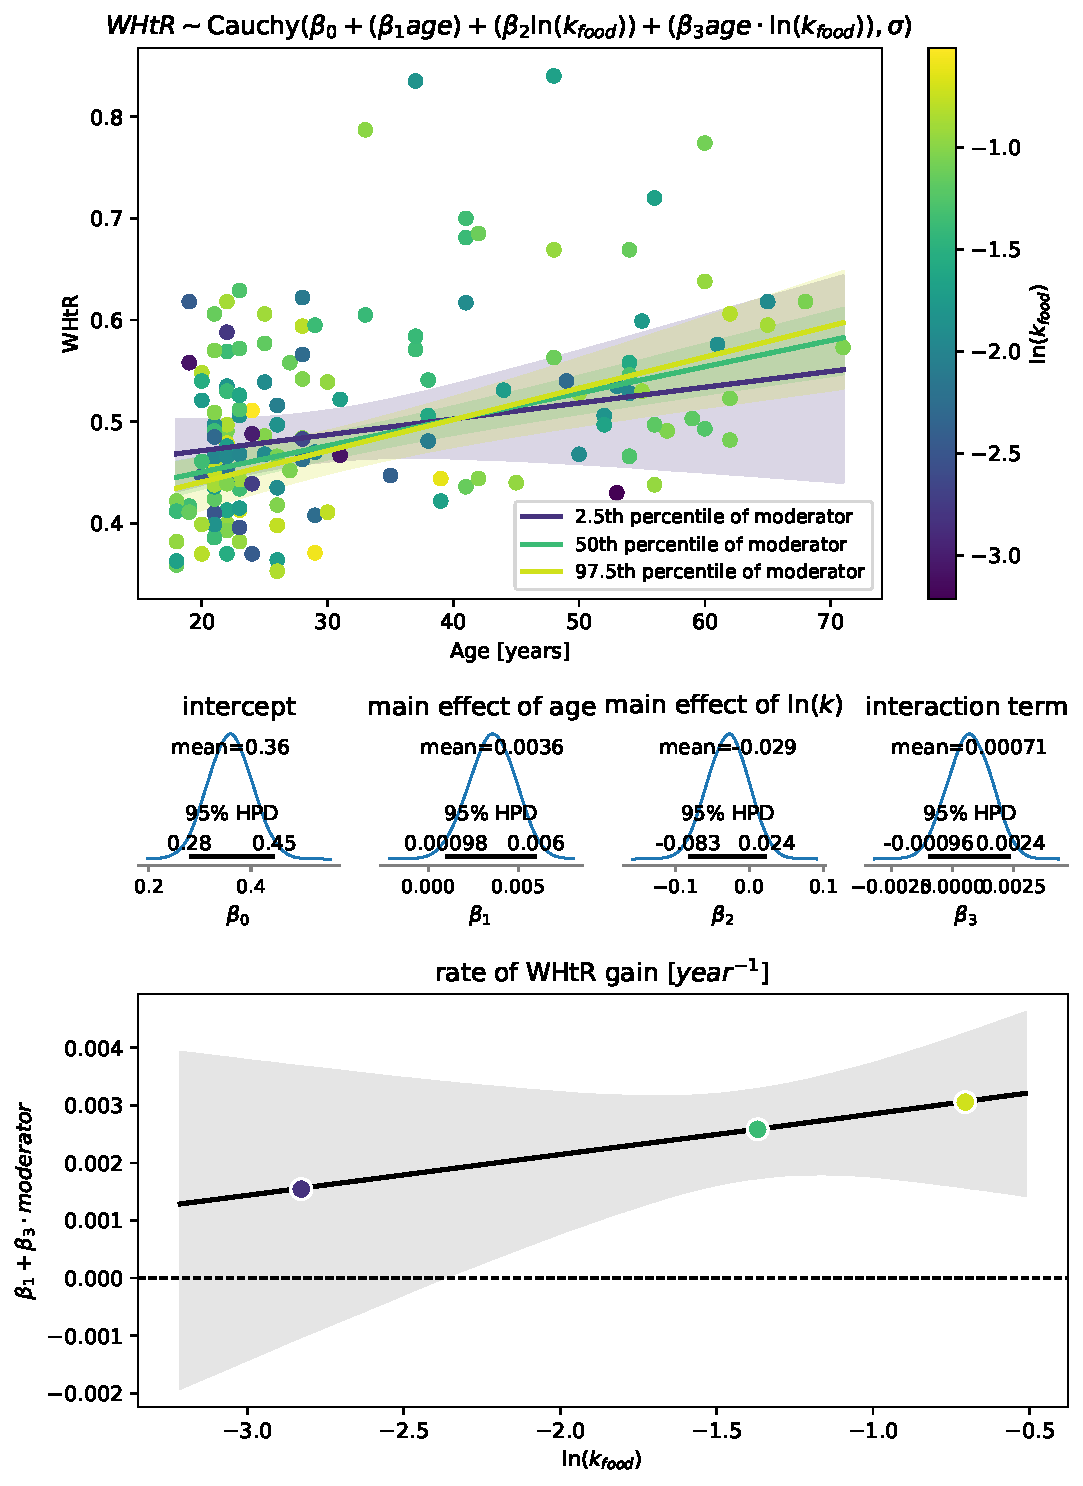
\includegraphics[width=0.8\textwidth]{analysis/study2 whtr~age*food.pdf} 
	\caption{Bayesian moderation analysis for Study 2 with age and discounting of food in predicting WHtR.}
	\label{fig:s2_whtr_food}
\end{figure*}


% REANALYSIS ==============================

\begin{figure*} 
	\centering
	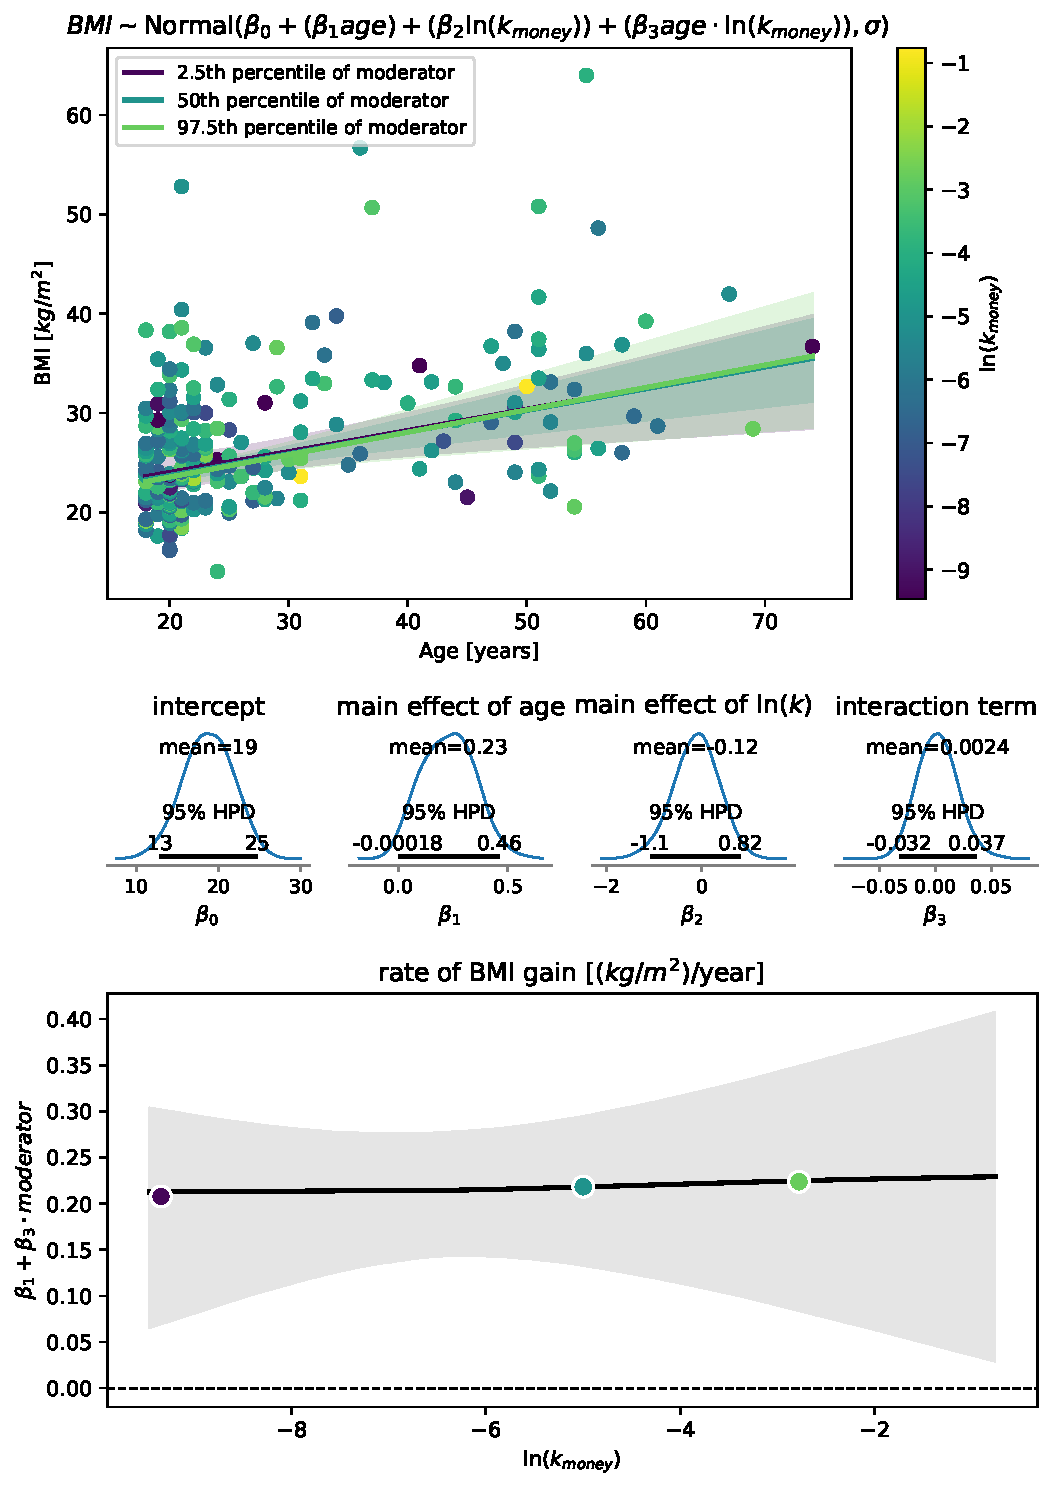
\includegraphics[width=0.8\textwidth]{veillard_vincent_2020_reanalysis/veillard_vincent_reanalysis_money.pdf} 
	\caption{Bayesian moderation analysis for the reanalysis of data from \cite{VeillardVincent2020} with age and discounting of money in predicting BMI.}
	\label{fig:vv_money}
\end{figure*}

\begin{figure*} 
	\centering
	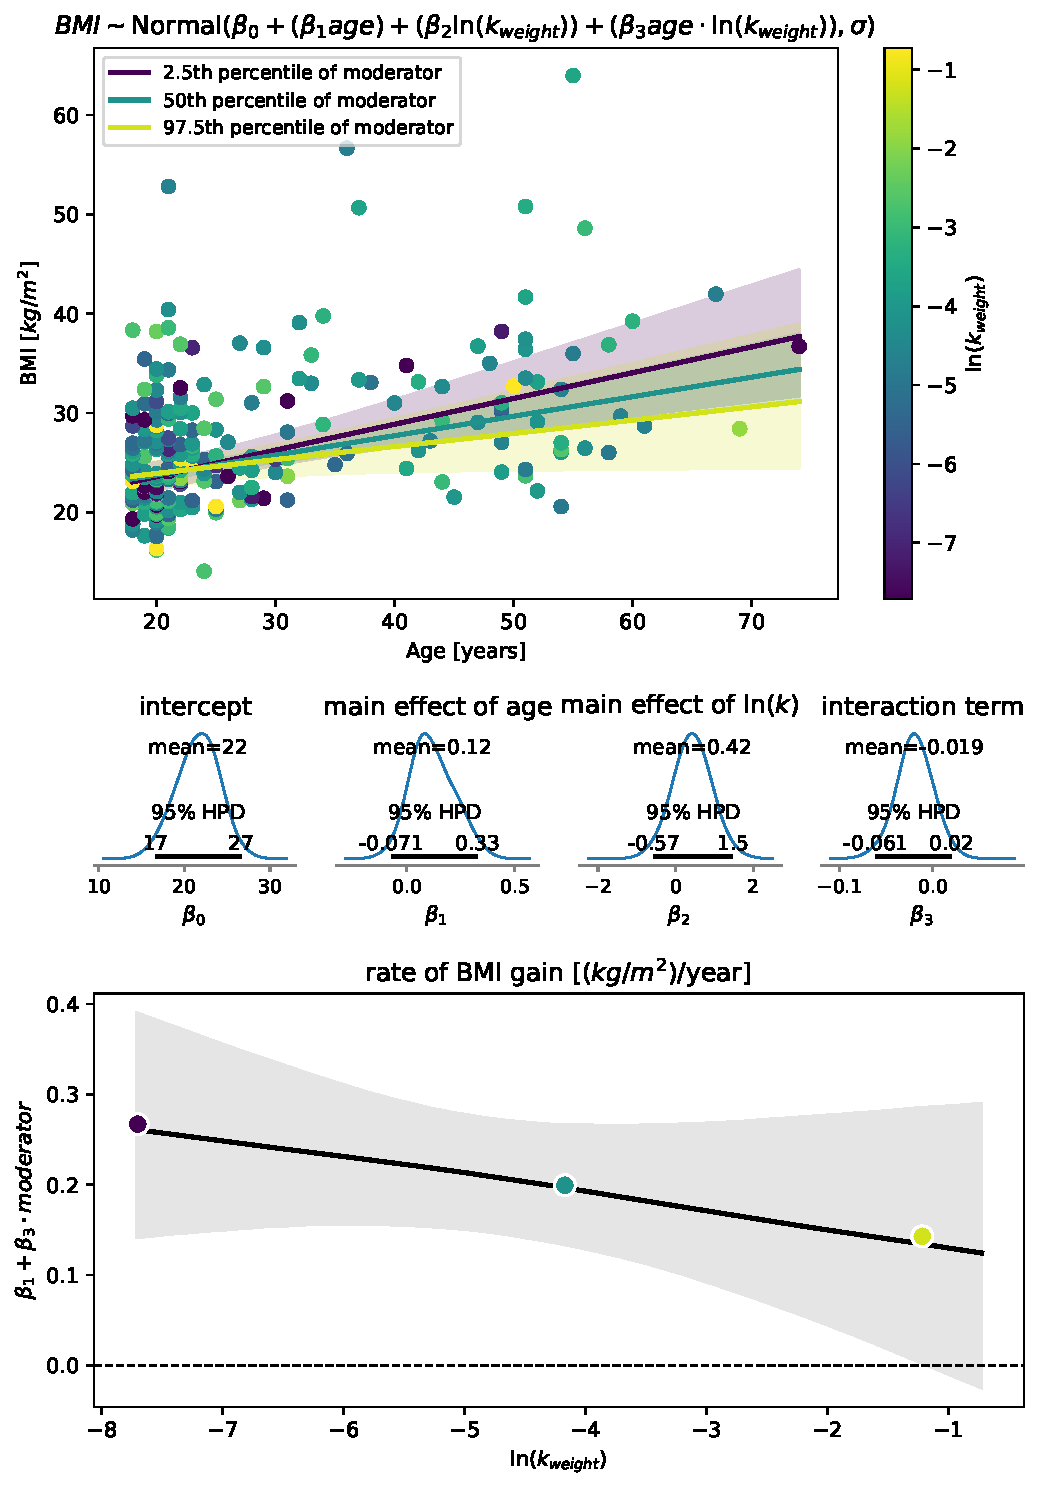
\includegraphics[width=0.8\textwidth]{veillard_vincent_2020_reanalysis/veillard_vincent_reanalysis_weight.pdf} 
	\caption{Bayesian moderation analysis for the reanalysis of data from \cite{VeillardVincent2020} with age and discounting of money in predicting BMI.}
	\label{fig:vv_money}
\end{figure*}

\begin{figure*} 
	\centering
	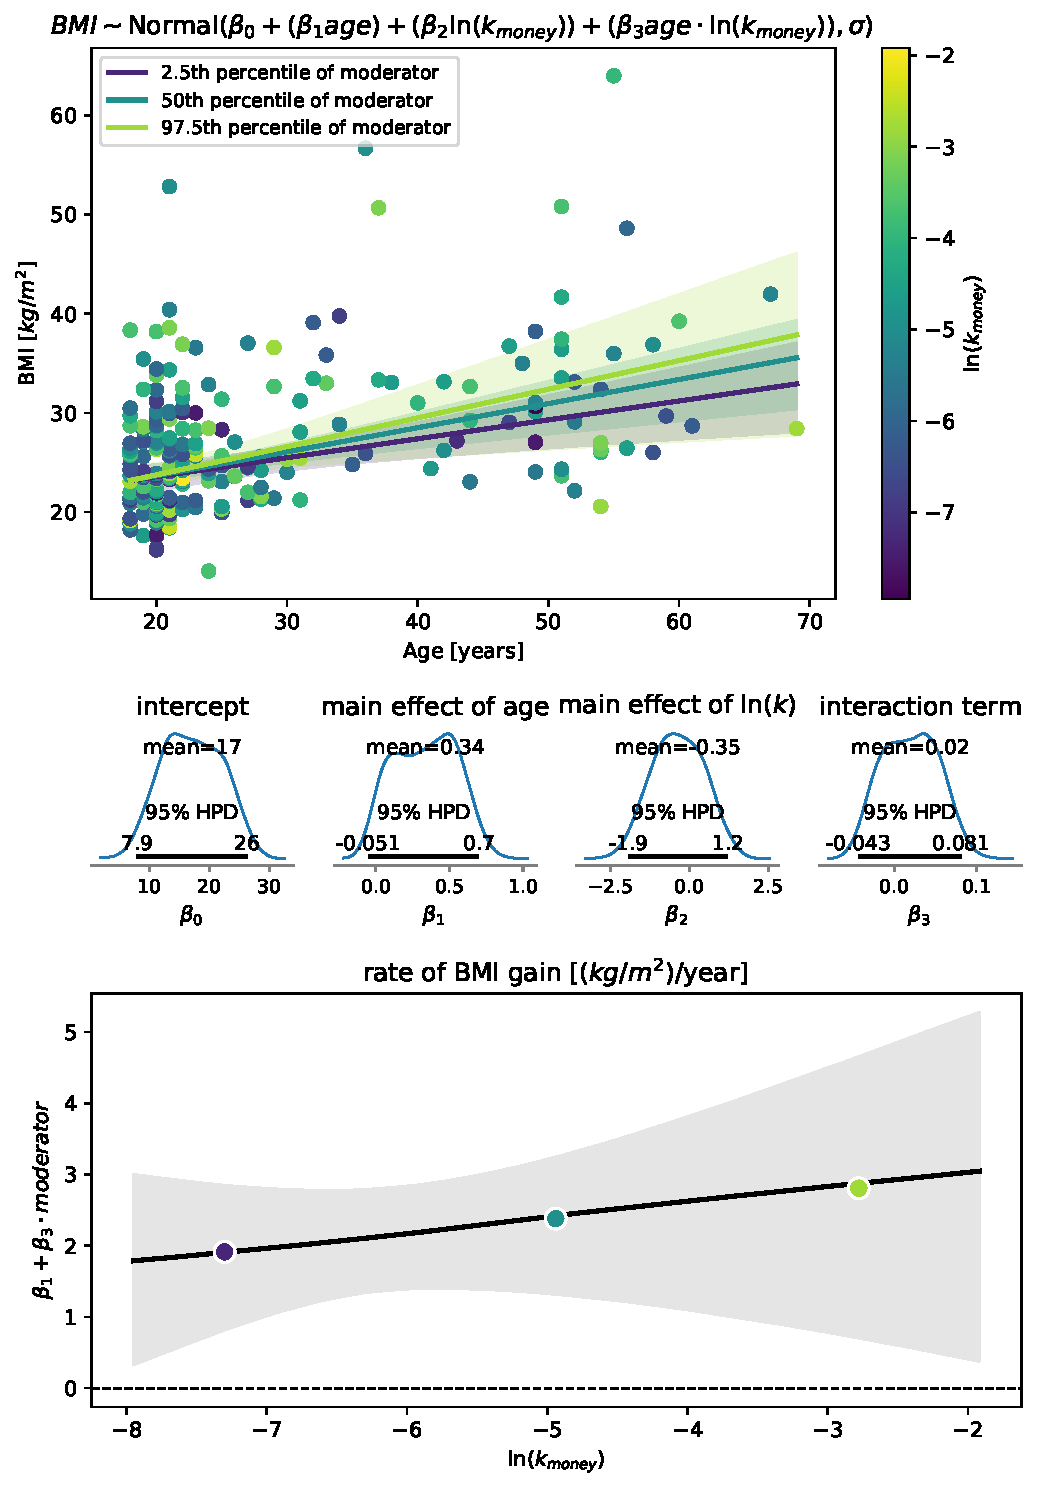
\includegraphics[width=0.8\textwidth]{veillard_vincent_2020_reanalysis/veillard_vincent_reanalysis_truncated_money.pdf} 
	\caption{Bayesian moderation analysis for the reanalysis of data from \cite{VeillardVincent2020} with age and discounting of money in predicting BMI. For this analysis, discount rates were truncated outside of the sensitive rate.}
	\label{fig:vv_money_trunc}
\end{figure*}

\begin{figure*}
	\centering
	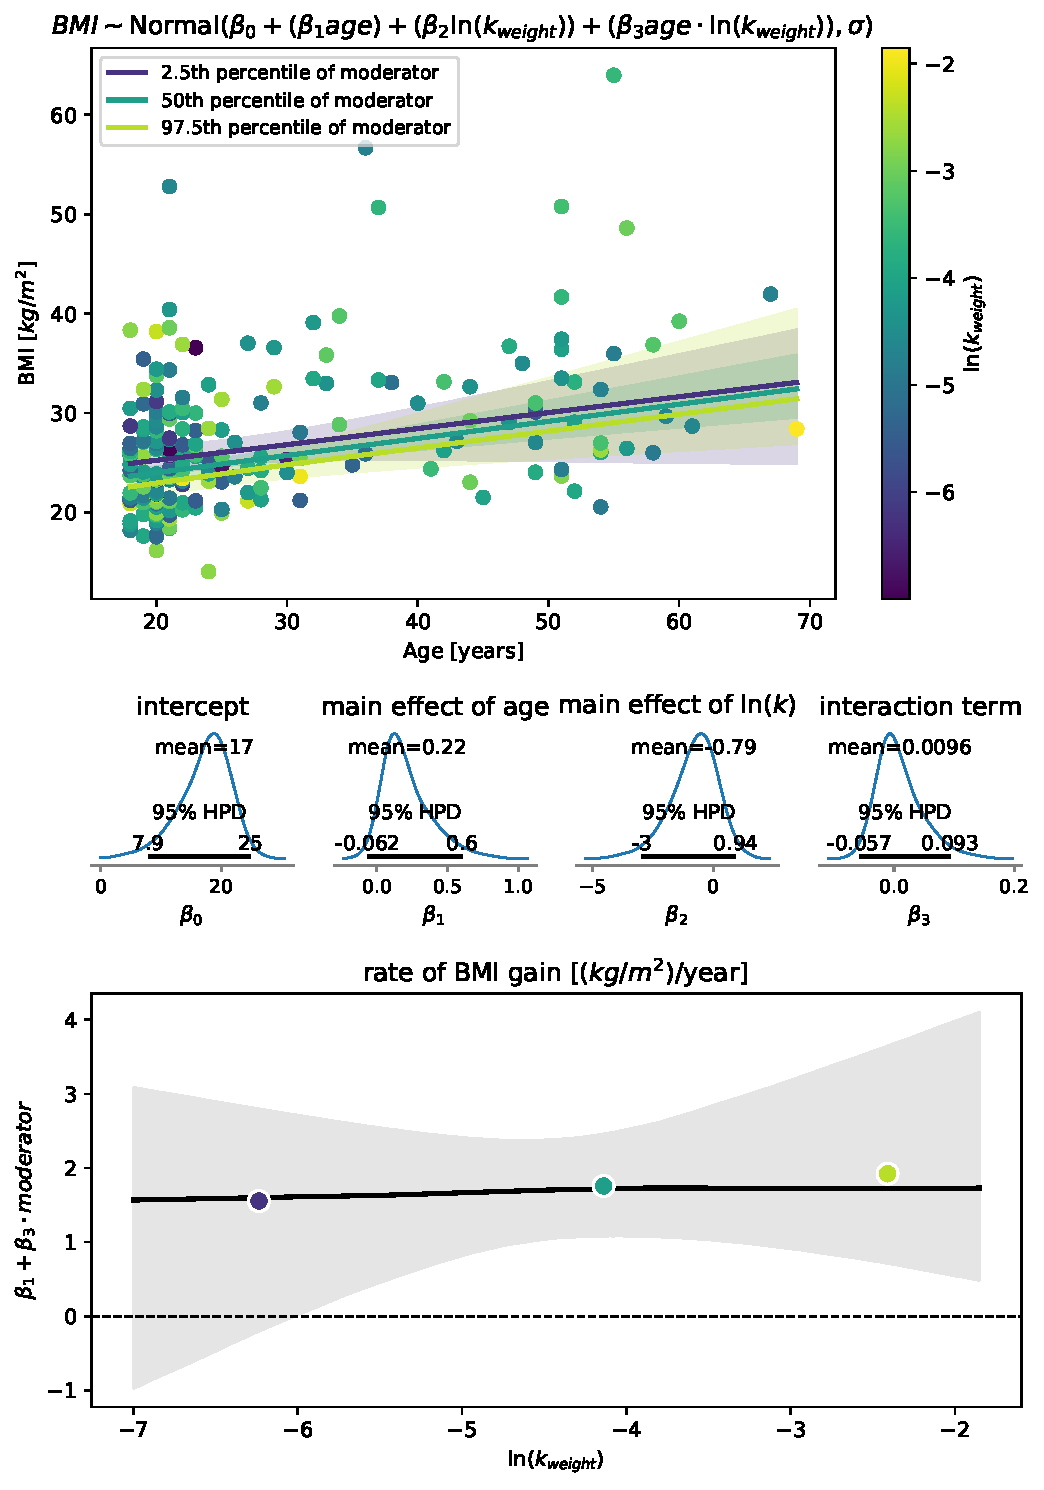
\includegraphics[width=0.8\textwidth]{veillard_vincent_2020_reanalysis/veillard_vincent_reanalysis_truncated_weight.pdf} 
	\caption{Bayesian moderation analysis for the reanalysis of data from \cite{VeillardVincent2020} with age and discounting of money in predicting BMI. For this analysis, discount rates were truncated outside of the sensitive rate.}
	\label{fig:vv_money_trunc}
\end{figure*}


% META ANALYSIS ===========================================


\begin{figure*} 
	\centering
	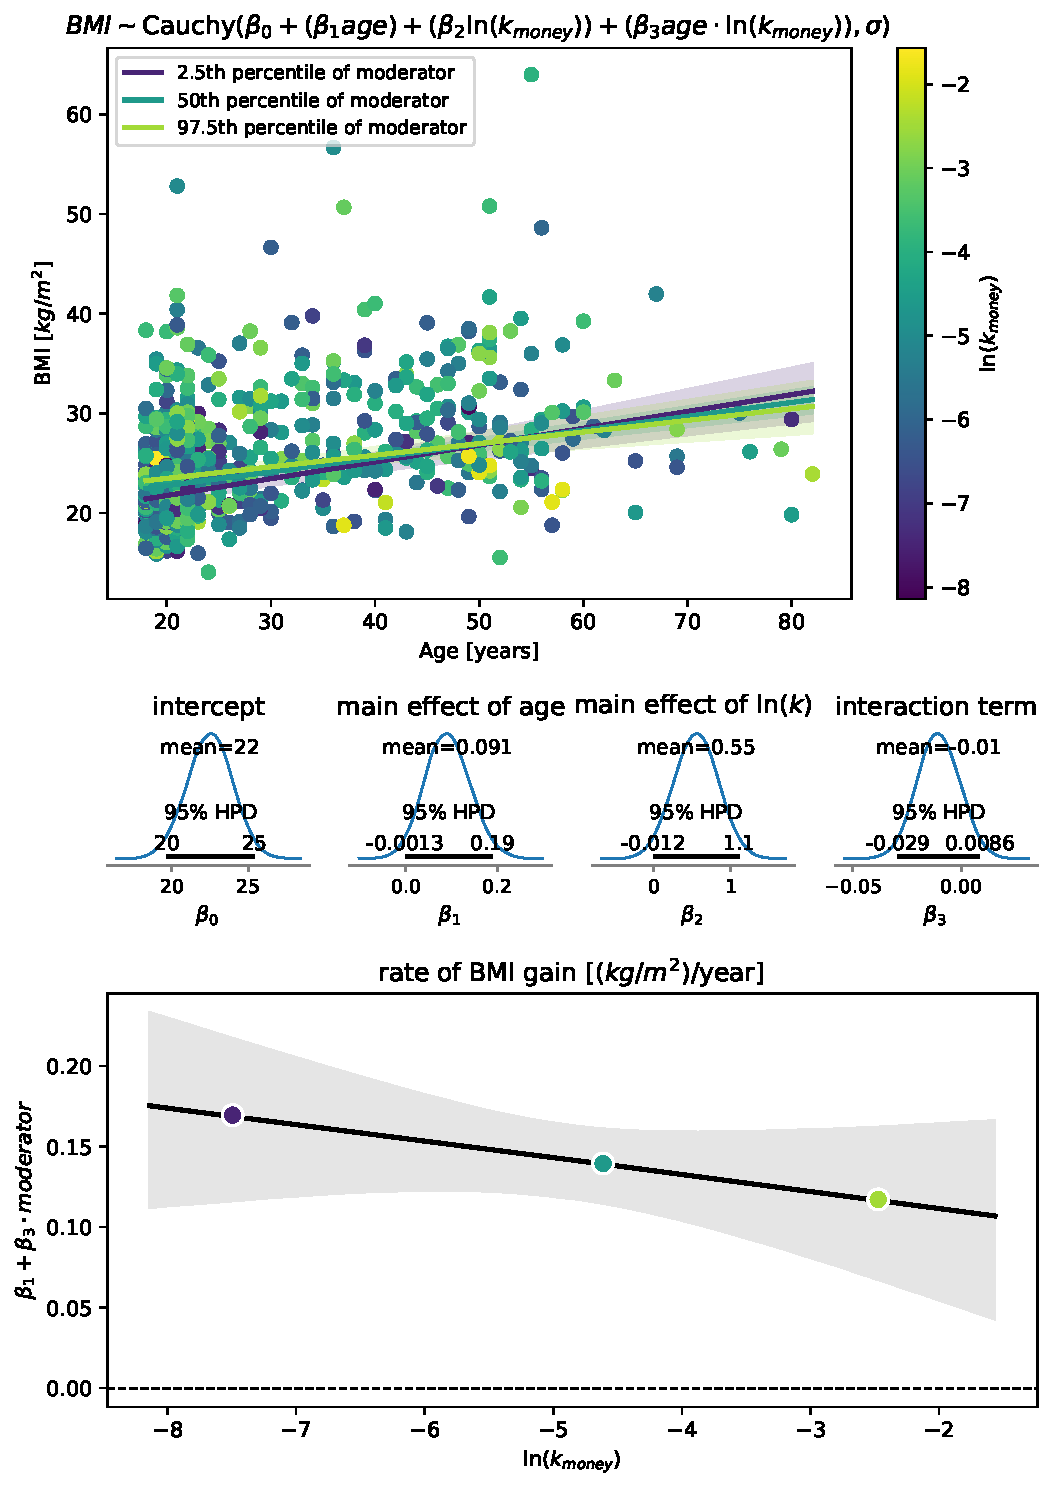
\includegraphics[width=0.8\textwidth]{meta_analysis/meta analysis bmi~age*money.pdf} 
	\caption{Bayesian moderation analysis for discounting of money. Data pooled over \cite{VeillardVincent2020} and Study1.}
	\label{fig:meta_money}
\end{figure*}

\begin{figure*} 
	\centering
	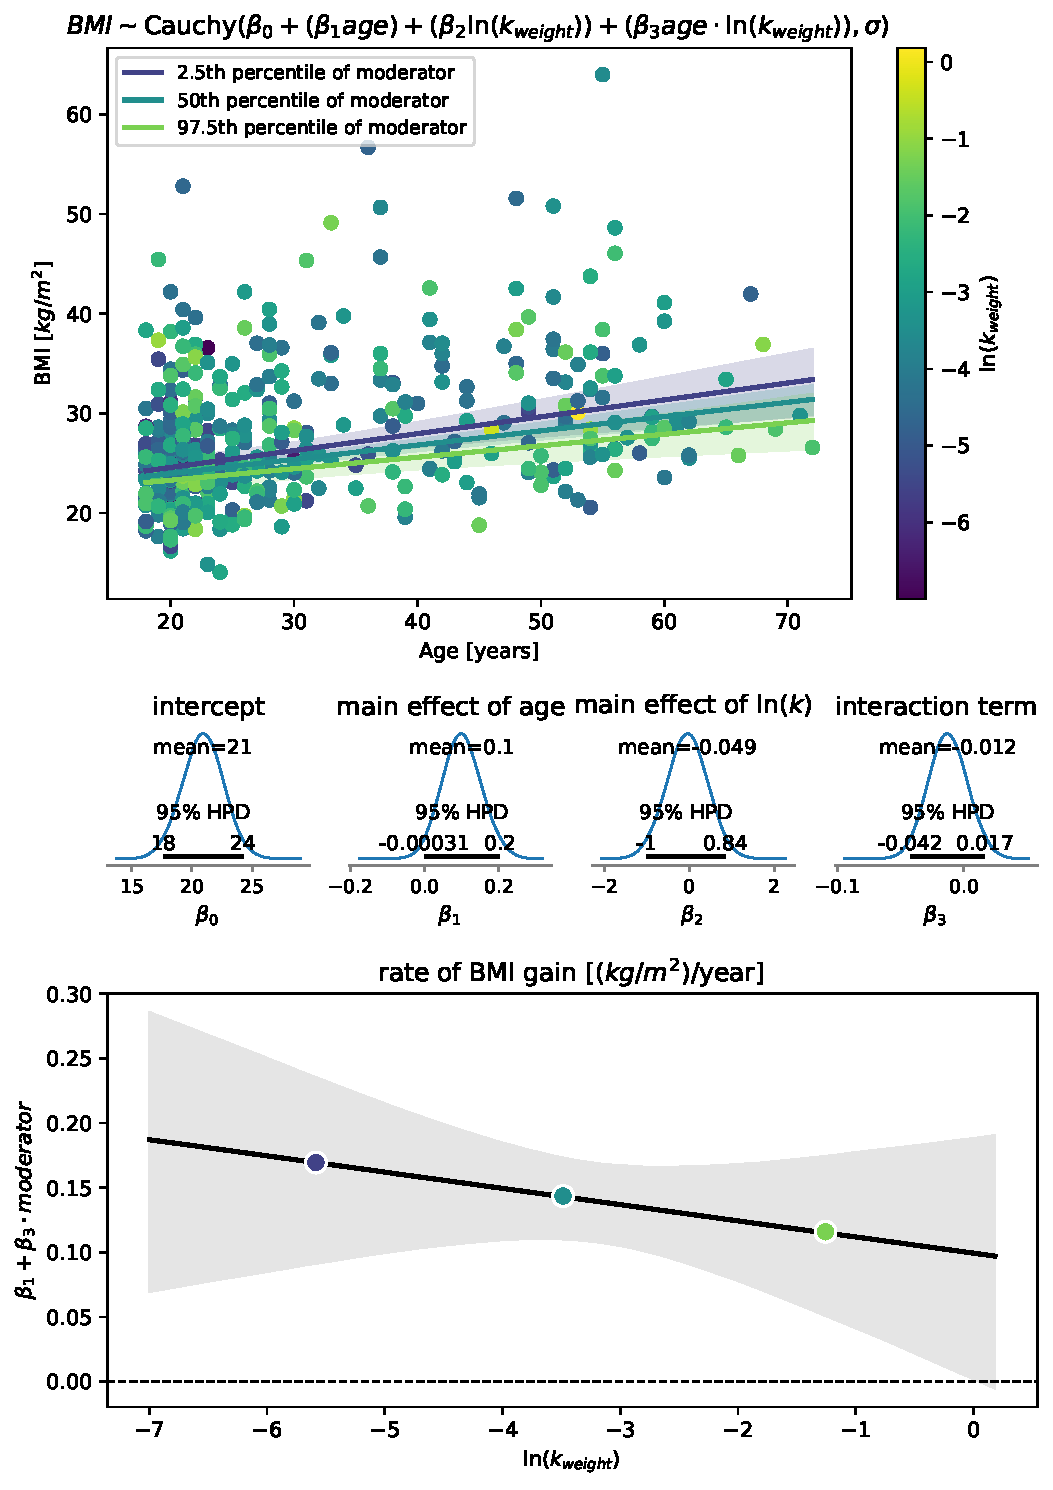
\includegraphics[width=0.8\textwidth]{meta_analysis/meta analysis bmi~age*weight.pdf} 
	\caption{Bayesian moderation analysis for discounting of weight loss. Data pooled over \cite{VeillardVincent2020} and Study2.}
	\label{fig:meta_weight}
\end{figure*}

\begin{figure*} 
	\centering
	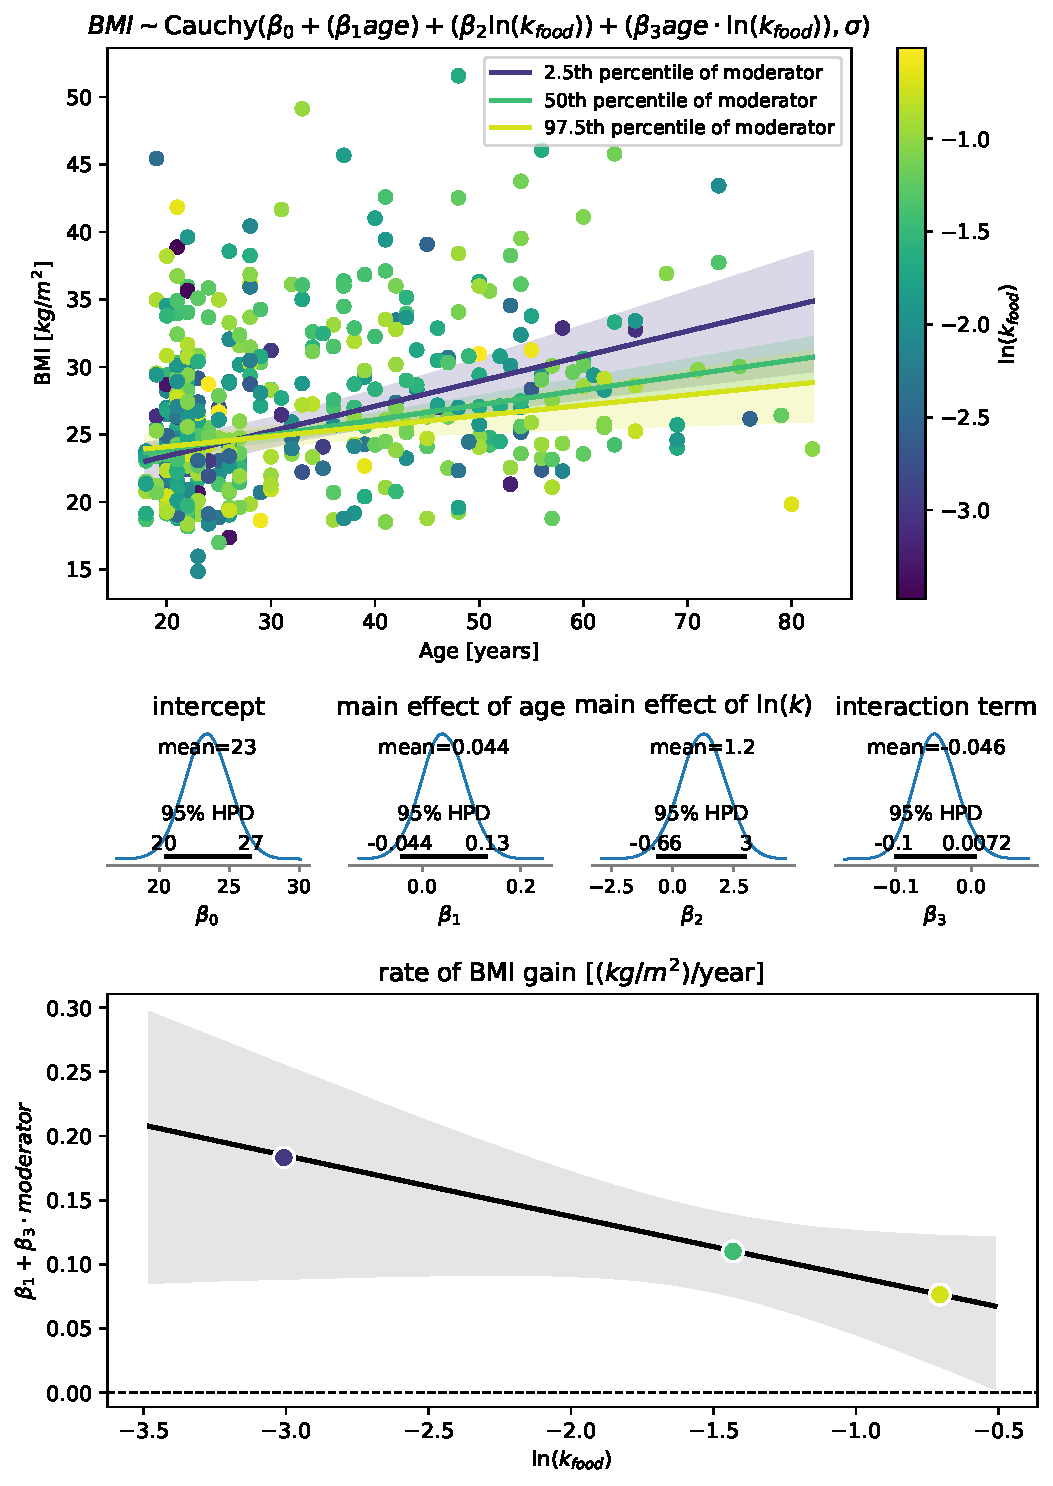
\includegraphics[width=0.8\textwidth]{meta_analysis/meta analysis bmi~age*food.pdf} 
	\caption{Bayesian moderation analysis for discounting of food. Data pooled over Study 1 and Study2.}
	\label{fig:meta_food}
\end{figure*}


% =========================================================
\bibliographystyle{apacite}
\bibliography{supplementary_references.bib}


\end{document}